\documentclass[a4paper,10pt,twoside]{report}

%ifdef PDF
%\usepackage[pdftex,colorlinks]{hyperref}
%endif

\usepackage[T1]{fontenc}
\usepackage[latin1]{inputenc}
\usepackage[ngerman]{babel}
%\usepackage[english]{babel}
\usepackage{ngerman,graphicx,float,latexsym,textcomp,longtable,verbatim,dsfont}

\setlength{\oddsidemargin}{1cm}
\setlength{\evensidemargin}{0cm}
\setlength{\textwidth}{15cm}

\pagestyle{headings}

%
%
% Includes
%
%%%%%%%%%%%
%\includeonly{title, intro, glossary}
%\includeonly{title, gisdb, app_gisdb, glossary}
%\includeonly{title, spatial, glossary}
%\includeonly{title, webservice, app_webservice, glossary}
%\includeonly{title, compreh, glossary}
%\includeonly{title, gisdb, webservice, app_gisdb, glossary}
%\includeonly{title, intro, gisdb, webservice, app_gisdb, app_webservice, glossary}

% Neue Umgebungen und Definitionen
%
%%%%%%%%%%%%%%%%%%%%%%%%%%%%%%%%%%%
%
% Hilfsdefinitionen
%%%%%%%%%%%%%%%%%%%
% der Betreuer soll den Abschnitt durchlesen
\newenvironment{lesen}%
{\vspace{5mm}\begin{sloppypar}
  \noindent\hrulefill\, BEGINN \,\hrulefill
  \end{sloppypar}
}%
{\begin{sloppypar}
  \noindent\hrulefill\, ENDE   \,\hrulefill
  \end{sloppypar}\vspace{5mm}
}

% der Betreuer soll den Abschnitt unter der Frage #1 durchlesen und
% kommentieren
\newenvironment{kommentar}[1]%
{\vspace{5mm}
  \begin{sloppypar}\noindent\hrulefill\, BEGINN Kommentar \,\hrulefill

  {\noindent\it #1}
  \end{sloppypar}
}%
{\begin{sloppypar}
  \noindent\hrulefill\, ENDE Kommentar   \,\hrulefill
  \end{sloppypar}\vspace{5mm}
}

% Frage an den Betreuer
\newcommand{\frage}[1]{\vspace{10mm}
\begin{sloppypar}{\bf Frage:} #1\end{sloppypar}
\vspace{10mm}}

% Bemerkung f�r den Betreuer
\newcommand{\bemerkung}[1]{\vspace{5mm}
\begin{sloppypar}{\bf Bemerkung:} #1\end{sloppypar}
\vspace{5mm}}

%%%%%%%%%%%%%%%%%%%%%%%%%%
% notwendige Definitionen
%%%%%%%%%%%%%%%%%%%%%%%%%%
\newtheorem{theorem}{Theorem}[chapter]
\newtheorem{lemma}{Lemma}[chapter]
\newtheorem{definition}{Definition}[chapter]
\newtheorem{beispiel}{Beispiel}[chapter]

% Beweis-Umgebung
\newenvironment{beweis}{\noindent {\bf Beweis:}}{\hfill$\Box$\smallskip}

% Numerierung von enumerate beginnt auf dem ersten Level mit Buchstaben
\renewcommand{\labelenumi}{(\alph{enumi})}
\renewcommand{\labelenumii}{(\roman{enumii})}

% Abk�rzungen
\newcommand{\lt}{$<$}
\newcommand{\gt}{$>$}
\newcommand{\ul}{\underline}
\newcommand{\ol}{\overline}
\newcommand{\zB}{z.\,B.\ }

% Trademarks
\newcommand{\multinet}{MultiNet{\small\texttrademark} }
\newcommand{\esri}{ESRI\raisebox{1ex}{\tiny\textregistered} }
\newcommand{\ibm}{IBM\raisebox{1ex}{\tiny\textregistered} }
\newcommand{\dbZ}{DB2\raisebox{1ex}{\tiny\textregistered} }

% Titel der Arbeit
\newcommand{\titel}{Tolle Teile Tauchen Tief}
%
% Beginn
%
%%%%%%%%%
\begin{document}

\begin{titlepage}
\hspace{0cm}
\vspace{-2cm}
 
\begin{flushright}

\includegraphics[width=3.2 cm]{bilder/husiegel.pdf}
\end{flushright}
 
 
\begin{center}
  \vspace{0.5 cm}
  \LARGE{\bf Ein dezentrales Transitionssystem zur Manipulation von geteilten Wörtern einer regulären Sprache} \\ % Hier fuegen Sie den Titel Ihrer Arbeit ein.
  \vspace{1 cm}
  \LARGE  Bachelorarbeit \\ % Geben Sie anstelle der Punkte an, ob es sich um eine
                % Diplomarbeit, eine Masterarbeit oder eine Bachelorarbeit handelt.
  \vspace{1cm}
  \Large zur Erlangung des akademischen Grades \\
  Bachelor of Science (B. Sc.) \\ % Bitte tragen Sie hier anstelle der Punkte ein:
         % Diplominformatiker(in),
         % Bachelor of Arts (B. A.),
         % Bachelor of Science (B. Sc.),
         % Master of Education (M. Ed.) oder
         % Master of Science (M. Sc.).
  \vspace{1.0cm}
  {\large
    \bf{
      \scshape
      Humboldt-Universit\"at zu Berlin \\
      Institut f\"ur Informatik\\
    }
  } 
  % \normalfont
\end{center}
\vspace{1.0 cm}
{\large
  \begin{tabular}{llll}
    eingereicht von:    & Denis Erfurt && \\ % Bitte Vor- und Nachnamen anstelle der Punkte eintragen.
    geboren am:         & 02.04.1988 && \\
    in:                 & Novosibirsk && \\
    &&&\\
    Gutachter(innen): & Prof. Dr. Klaus Reinhardt && \\
              & Prof. Dr. Jens-Peter Redlich && \\% Bitte Namen der Gutachter(innen) anstelle der Punkte eintragen
    &&&\\
    eingereicht am:     & \dots\dots \hspace{3cm} verteidigt am: & & \dots\dots \\ % Bitte lassen Sie
                                    % diese beiden Felder leer.
                                    % Loeschen Sie ggf. das letzte Feld, wenn
                                    % Sie Ihre Arbeit laut Pruefungsordnung nicht
                                    % verteidigen muessen.
  \end{tabular}
}
 
\end{titlepage}


% \thispagestyle{empty} % Seite hinter dem Titelblatt hat keine Seitennummer
% \cleardoublepage

\pagenumbering{roman}
\tableofcontents
% \listoffigures
% \listoftables

% \cleardoublepage

\chapter{Einleitung}
\pagenumbering{arabic}

Nach einem langen Spaziergang durch die Innenstadt von K�ln steht eine
Touristin vor dem Dom und m�chte mit den �ffentlichen Verkehrsmitteln wieder
zur�ck in ihr Hotel. Sie greift zum Mobiltelefon und stellt eine Verbindung
zum WAP-Portal ihres Mobilfunkanbieters her. Nach der Auswahl des Men�punktes
{\em �ffentliche Verkehrsmittel} �ffnet sich eine Eingabemaske, in dem
sie ihr Ziel, den Namen ihres Hotels, eingibt. Kurze Zeit sp�ter wird eine
Wegbeschreibung zur n�chstgelegenen Bushaltestelle sowie die Fahrverbindung
zu ihrem Hotel auf dem Display angezeigt.

Insgesamt realisiert das entworfene Szenario einen standortbezogenen Dienst
(Location Based Service). Unter Ausnutzung der Ortbarkeit eines eingeschalteten
Mobiltelefons lassen sich auf die momentane Position abgestimmte Dienste
und Informationen anbieten. F�r die Realisierung eines solchen Szenarios ist
ein Zusammenf�hren verschiedenster Datenquellen erforderlich.

\bigskip

\begin{figure}[htbp]
  \centering
  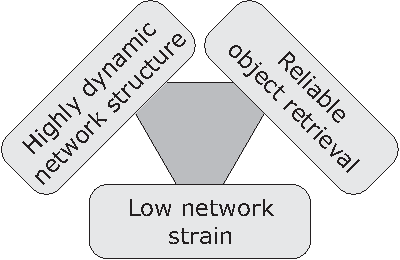
\includegraphics{picture/tradeoff}
  \caption{Tradeoffs in P2P systems}
  \label{fig:tradeoff}
\end{figure}

So beginnt zum Beispiel eine Studienarbeit. Nicht vergessen, hier in der Einleitung auch einen �berblick �ber die einzelnen Kapitel der Arbeit sowie deren Inhalt zu geben! So kann man z.B. mittels \texttt{ref} auf Verweise innerhalb des Dokumentes verweisen, wenn diese mit \texttt{label} vorher definiert wurden. Hier zum Beispiel ein Verweis auf das erste Kapitel im Anhang \ref{app:c1:s1} oder hier einer auf das nun folgende Bild \ref{fig:tradeoff}.

Ganz wichtig sind nat�rlich auch Zitate. Nat�rlich wird daf�r BibTeX verwendet, doch was man daf�r wissen muss, beschr�nkt sich auf relativ wenig: Anlegen und Pflegen einer .bib - Datei, am besten mit dem sehr guten Tool JabRef und zitieren im Text mit \texttt{cite}. So kann man dann beweisen, dass sich in einem Artikel \cite{Herschel2003} �ber Goya ge�u�ert wurde.

\chapter{Inhalt}
Im Inhalt steht dann die eigentlich Arbeit. Insbesondere kann man einige der in main.tex definierten Umgebungen benutzen. Siehe hier:

\section{Umgebungen f�r den Betreuer}

\subsection{lesen}
\begin{lesen}
Dies hier ist neuer Text, der Betreuer soll den Abschnitt hier dezidiert durchlesen.
\end{lesen}

\subsection{kommentar}
\begin{kommentar}{Halten Sie den Einfluss der Variablen auf den Gesamtkontext f�r relevant oder ist das ein Me�fehler?}
Dies ist der Text, auf den sich die Frage bezieht. Der Betreuer soll den Abschnitt unter der Frage durchlesen und kommentieren.
\end{kommentar}

\subsection{frage}
W�hrend man so Text schreibt, stellt sich einem vielleicht eine wichtige Frage, die man jetzt oder sp�ter noch beantwortet wissen will.
\frage{Warum schreibe ich das eigentlich?}

Analog funktioniert eine Bemerkung, die man dem Betreuer mit auf dem Weg geben m�chte: \bemerkung{Ich finde diesen Abschnitt sehr gelungen!}

\section{Umgebungen f�r den Schreiber}

F�r den Schreiber einer Arbeit am Institut f�r Informatik werden hier ein paar Umgebungen definiert, deren Nummerierung dann sinnvoll von \LaTeX mitgez�hlt wird.

\begin{theorem}
\label{theorem:mann}
Ein Mann, der eine Grube gr�bt, f�llt selbst hinein.
\end{theorem}

Dies l��t sich dann sp�ter auch noch gut referenzieren. Siehe f�r eine so richtig gut gelungene Referenzierung \zB diese Referenzierung hier, welche auf das obige Theorem \ref{theorem:mann} verweist.

Analog funktionieren lemma, definition, beispiel.

\begin{lemma}
Theorem \ref{theorem:mann} gilt genau dann wenn die Grube tief genug ist.
\end{lemma}

Ein konkreter Beweis wird nicht nummeriert und steht daher als einfache \LaTeX - Umgebung mitten in der Welt herum.

\begin{beweis}
Ist die Grube nicht tief, kann man nicht von fallen sprechen. Theorem \ref{theorem:mann} kann daher nicht gelten.
\end{beweis}

Der Vollst�ndigkeit halber sei hier noch eine kleine Tabelle gerendert:

\begin{table}[htbp]
\centering
\begin{tabular}{lcccl}
\hline
$P_1$           & $\Rightarrow$ & $O_{Job}$           & $\Leftarrow$ & $P_3$ \\ \hline
Jobs            & $\rightarrow$ & job:jobPosition     & $\leftarrow$ & IT\_Job \\
job\_desc       & $\rightarrow$ & job:description     & $\leftarrow$ & position \\
organization    & $\rightarrow$ & job:organization    & $\leftarrow$ & company \\
                &               & job:department      & $\leftarrow$ & department \\
start\_date     & $\rightarrow$ & job:start\_date     & $\leftarrow$ & begin \\
naics           & $\rightarrow$ & job:naics           &              & \\
                &               & job:publish\_date   & $\leftarrow$ & published \\\hline
\end{tabular}
\caption{Example mapping of $P_1$ and $P_2$ to a sample job ontology}
\label{tab:ex_mapping}
\end{table}


% \begin{appendix}
\chapter{Erster Bereich des Anhangs}
In diesem Bereich beginnt der Anhang. Man kann auch im Anhang eine Unterteilung nach Abschnitten durchf�hren...
\section{Erster Abschnitt}
\label{app:c1:s1}
... wie hier leicht zu erkennen ist.
\section{Zweiter Abschnitt}
... oder hier.

\chapter{Zweiter Bereich des Anhangs}
Hier kommt dann noch ein weiteres Kapitel im Anhang!

\end{appendix}


\bibliography{literatur}
\bibliographystyle{alpha}

% \cleardoublepage
\thispagestyle{empty}

%%%%%%%%%%%%%%%%%%%%%%%%%%%%%%%%%%%%%%%%%%%%%%%%%%%%%%%%%%%%%%%%%%%%%%%%%%%%%%%%%%%%%%%%%%%%%%%%%%%%
%% Selbststaendigkeitserklaerung
%%%%%%%%%%%%%%%%%%%%%%%%%%%%%%%%%%%%%%%%%%%%%%%%%%%%%%%%%%%%%%%%%%%%%%%%%%%%%%%%%%%%%%%%%%%%%%%%%%%%

{\parindent 0cm
%%%%%%%%%%%%%%%%%%%%%%%%%%deutsche Version%%%%%%%%%%%%%%%%%%%%%%%%%%%%%%
  
  \subsection*{Selbst\"andigkeitserkl\"arung}
  Ich erkl\"are hiermit, dass ich die vorliegende Arbeit selbst\"andig verfasst 
  und nur unter Verwendung der angegebenen Quellen und Hilfsmittel angefertigt habe. 
  Weiterhin erkl\"are ich, eine ...arbeit in diesem Studiengebiet erstmalig einzureichen.\\
%statt der Punkte Diplom, Master oder Bachelor angeben
  \vspace{3\baselineskip}
  
  Berlin, den \today \hspace{0.25\linewidth}\parbox{0.3\linewidth}{\dotfill}

%%%%%%%%%%%%%%%%%%%%%%%%%%englische Version%%%%%%%%%%%%%%%%%%%%%%%%%%%%%%%%%%%%%%%%%%%%%%%%%%%%%%%%%
\selectlanguage{english}
\subsection*{Statement of authorship}
I declare that I completed this thesis on my own and that information which has been 
directly or indirectly taken from other sources has been noted as such. Neither this 
nor a similar work has been presented to an examination committee.

  \vspace{3\baselineskip}
  
  Berlin, \today \hspace{0.25\linewidth}\parbox{0.3\linewidth}{\dotfill}
}



\end{document}
